\documentclass{article}

\usepackage[x11names]{xcolor}
\usepackage{pgfplots}

\begin{document}

\begin{equation}
f(x) = (x-5)^3-15(x-5)+50
\end{equation}

\begin{equation}
F(10) - F(0) = \int_0^{10} (x-5)^3-15(x-5)+50 \,\mathrm{d}x
\end{equation}


%\pgfplotsset{
%    integral segments/.code={\pgfmathsetmacro\integralsegments{#1}},
%    integral segments=3,
%    integral/.style args={#1:#2}{
%        ybar interval,
%        domain=#1+((#2-#1)/\integralsegments)/2:#2+((#2-#1)/\integralsegments)/2,
%        samples=\integralsegments+1,
%        x filter/.code=\pgfmathparse{\pgfmathresult-((#2-#1)/\integralsegments)/2}
%    }
%}
%
%\begin{tikzpicture}[/pgf/declare function={f=-15*(x-5)+(x-5)^3+50;},scale=0.8]
%\begin{axis}[
%    domain=0:10,
%    samples=100,
%    axis lines=middle,
%	ymax=100
%]
%\addplot [
%    fill=LightPink1!50!white, opacity=0.3 , draw=LightPink2,
%    integral segments=10,
%    integral=0:10
%] {f};
%\addplot [thick,draw=LightPink3] {f};
%\end{axis}
%\end{tikzpicture}
%\begin{tikzpicture}[/pgf/declare function={f=-15*(x-5)+(x-5)^3+50;},scale=0.8]
%\begin{axis}[
%    domain=0:10,
%    samples=100,
%    axis lines=middle,
%	ymax=100
%]
%\addplot [
%    fill=LightPink1!50!white, opacity=0.3 , draw=LightPink2,
%    integral segments=100,
%    integral=0:10
%] {f};
%\addplot [thick,draw=LightPink3] {f};
%\end{axis}
%\end{tikzpicture}
%

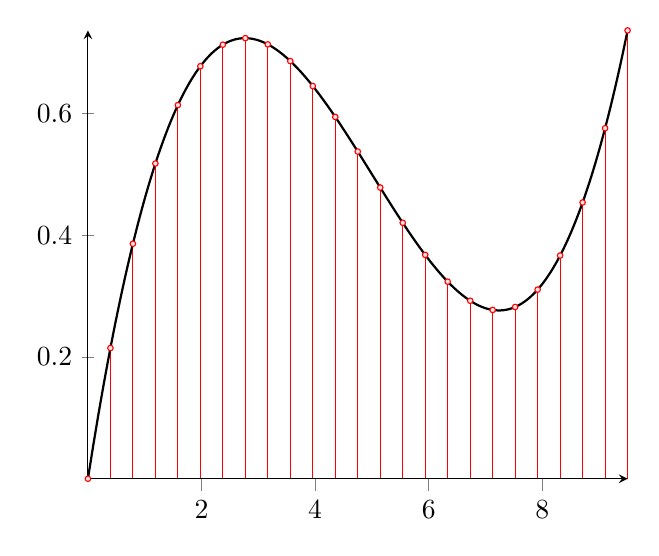
\begin{tikzpicture}
\begin{axis}[
%    xtick={0,1,3,5,7,9,11,13,15,17},ytick={0,...,1.5},
%    xmax=18,ymax=1.2,ymin=0,xmin=0,
%    enlargelimits=true,
    axis lines=middle,
    clip=false,
   % domain=0:17,
    axis on top,
ybar=1pt,
bar width=0pt,
/pgf/declare function={f=(-15*(x-5)+(x-5)^3+50)/100;}
    ]

\addplot [draw=red, fill=red!10,, samples=25, domain=0:9.5, mark=*, mark size=1pt] {f}\closedcycle;

\addplot[smooth, thick,domain=0:9.5,samples=101]{f};

\end{axis}
\end{tikzpicture}

\end{document}